\anglais
\doublespacing
\chapter{Supplementary material for \autoref{Foodweb}}

\section{SVD does not overfit on the European
network}\label{svd-does-not-overfit-on-the-european-network}

In order to ensure that the creation of the RDPG on the European network
does not lead to overfitting, we performed two numerical experiments.

First, we estimated the threshold that separates interactions from
non-interactions based on a decreasing amount of species; this
highlights that removing up to 50\% of the total species in the network
does not change the estimate of the threshold, suggesting that there is
an important amount of information contained in the first 12 ranks of
the network.

Second, we extracted \(\mathcal{L}\) and \(\mathcal{R}\), the left and
right subspace of the entire network, at rank 12. Then, for every number
\(n\) of interactions between 10 and \(\text{links}(M)-1\) (where \(M\)
is the European metaweb), we define \(m\) as a network in which \(n\)
interactions have either been randomly removed, randomly added, or both.
We then define \(\mathcal{l}\) and \(\mathcal{r}\) as the left and right
subspaces coming from the rank-12 RDPG applied to this network, and
compare the original network \(M\) to the one that was reconstructed
after thresholding \(\mathcal{l}\mathcal{r}\) by picking the cutoff that
maximizes Youden's \emph{J} measure (Youden, 1950).

This last experiment allows measuring the response of various measures
of fit of the binary classifier to incomplete sampling. We are
specifically interested in (i) the ability of RDPG to identify modified
interactions, (ii) the ability of RDPG to function as a performant
classifier in the presence of uncertainty in the original data, and
(iii) the ability of RDPG to reconstruct biologically realistic data
when interactions are withheld.

\subsection{Threshold estimation is robust to species
sub-sampling}\label{threshold-estimation-is-robust-to-species-sub-sampling}

In the initial experiment, we withheld an increasing number of species
from the European metaweb, ranging from 20\% for training and 80\% for
validation, to 90\% for training and 10\% for validation. Surprisingly,
the estimation of the threshold, here presented as the mean and standard
deviation of 50 folds for validation, is remarkably robust (and matches
the value obtained using the entire network, as a dashed line).
Specifically, even using 60\% of species to estimate the threshold gave
on average the same threshold as would be estimated based on the entire
network; therefore, this establishes that the decision in the main text
to use the entire European metaweb to set the threshold is correct.

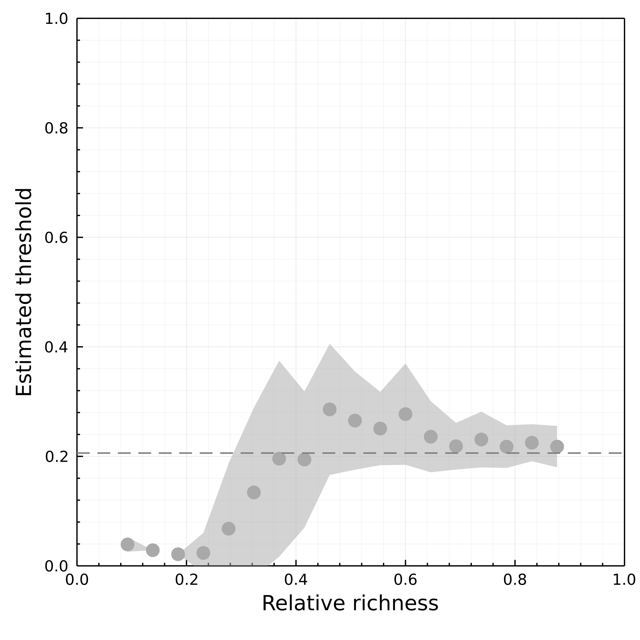
\includegraphics[width=\textwidth]{./figures/supplementary/sensibility_threshold_species.png}

More strikingly, looking at the rates of true/false positive/negative,
as illustrated below, it is clear that RDPG can be thresholded in a way
that yields an almost perfect classifier:

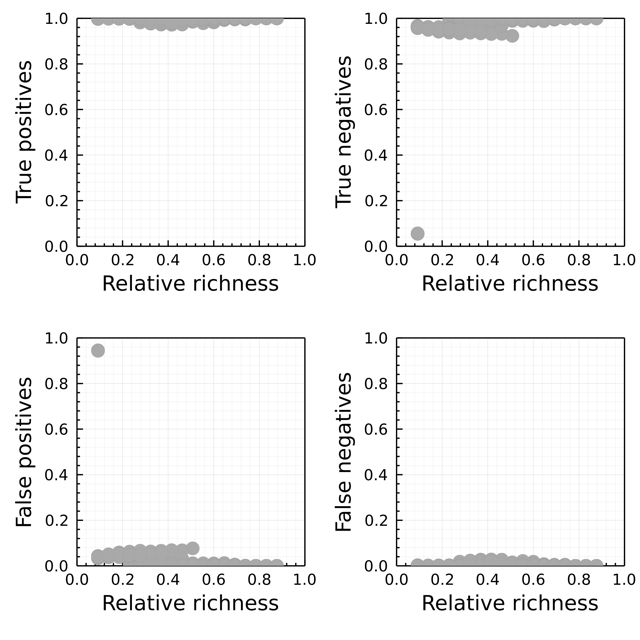
\includegraphics[width=\textwidth]{./figures/supplementary/sensibility_species.png}

These results may be surprising, given that ecological models usually do
not reach this degree of accuracy. That being said, we use the first 12
ranks of the network to approximate it, and this contains a lot of
information; in short, the minute discrepancies between the predictions
and the actual data can be attributed to leftover noise in the original
dataset.

\subsection{RDPG recovers withheld
interactions}\label{rdpg-recovers-withheld-interactions}

RDPG is able to correct almost all \emph{added} interactions (added
interactions were \emph{not} originally present in the European metaweb
and could be seen as introducing false positives to the data), which is
very strong evidence that the metaweb produced using it are not going to
contain too much spurious interactions. When \emph{removing}
interactions (\emph{i.e.} introducing false negatives to the data), even
when half are missing, RDPG was able to accurately reconstruct about 75
to 80\% of them. Predictably, the performance when both adding and
removing interactions is in between the two scenarios.

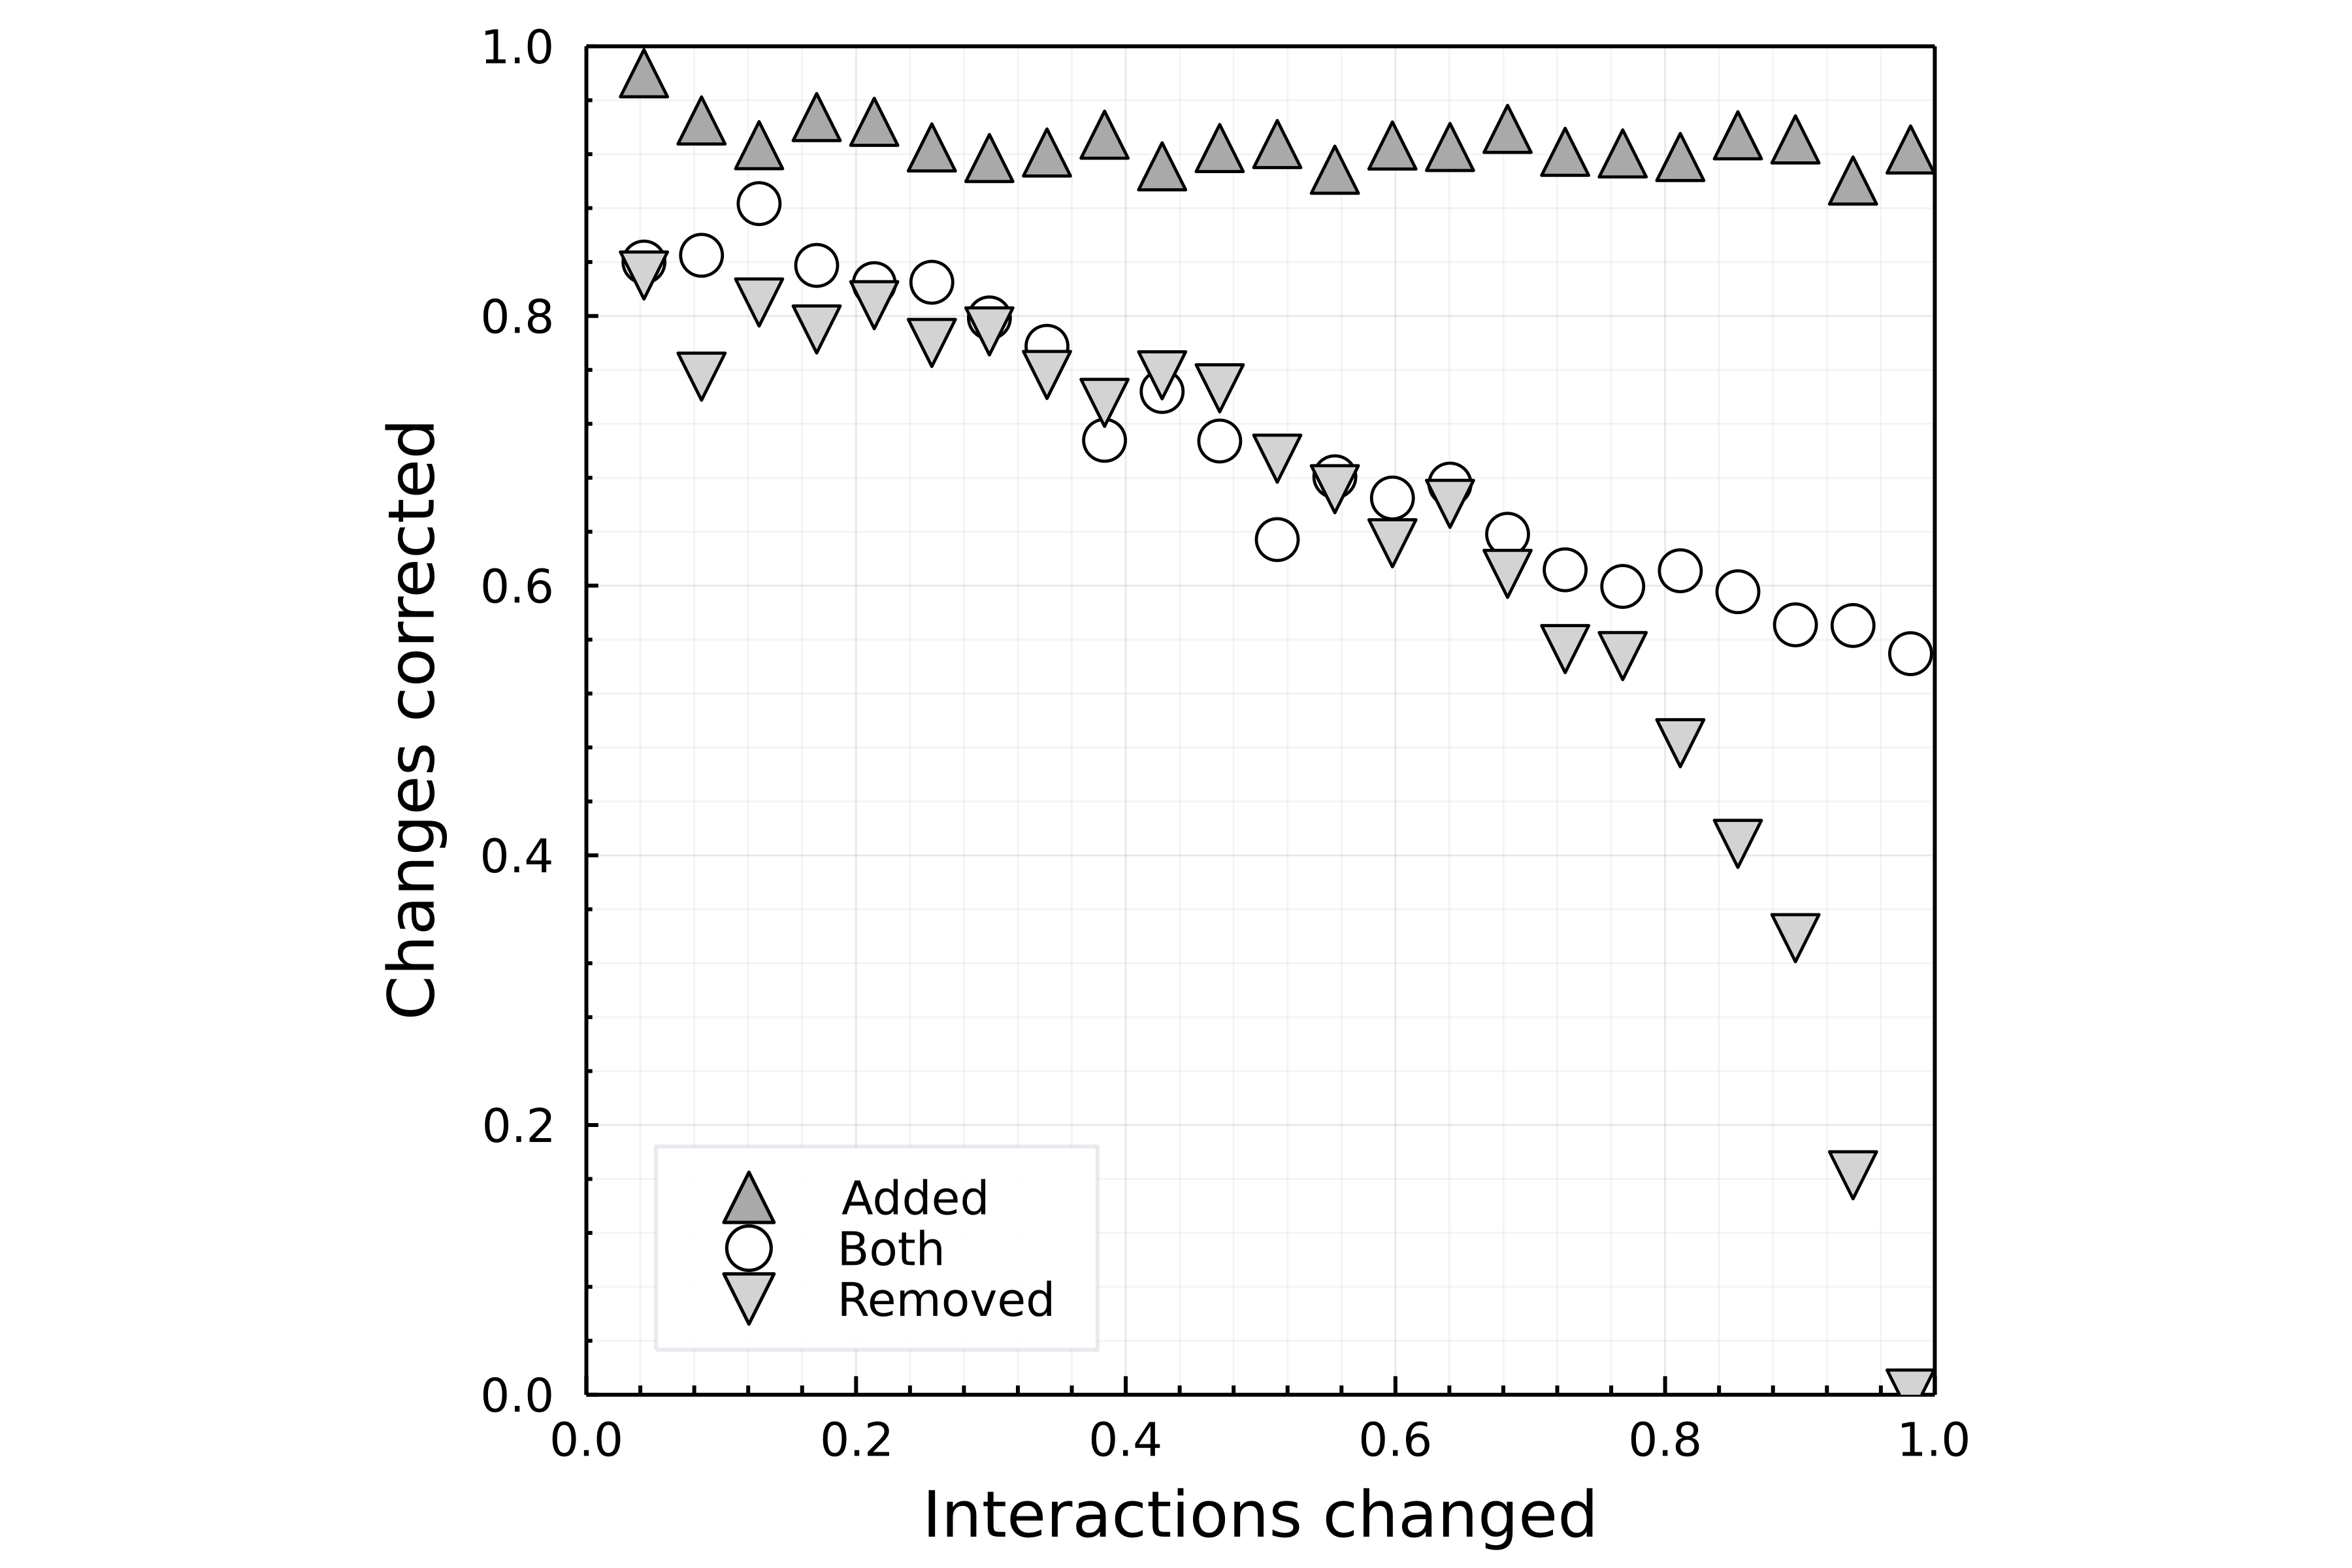
\includegraphics[width=\textwidth]{./figures/supplementary/sensibility_recovery.png}

The stochasticity in the proportion of recovered interactions is larger
when a small number of interactions are withheld, which makes sense as
the \emph{number} of interactions is far smaller (compared to the
overall network size).

Next, it is interesting to note that the threshold ``adapts'' to the
amount of missing information - the dashed line corresponds to the
threshold we used in the manuscript. Adding interactions specifically
did not result in an increase in the threshold, further suggesting that
RDPG is extremely good at removing spurious interactions.

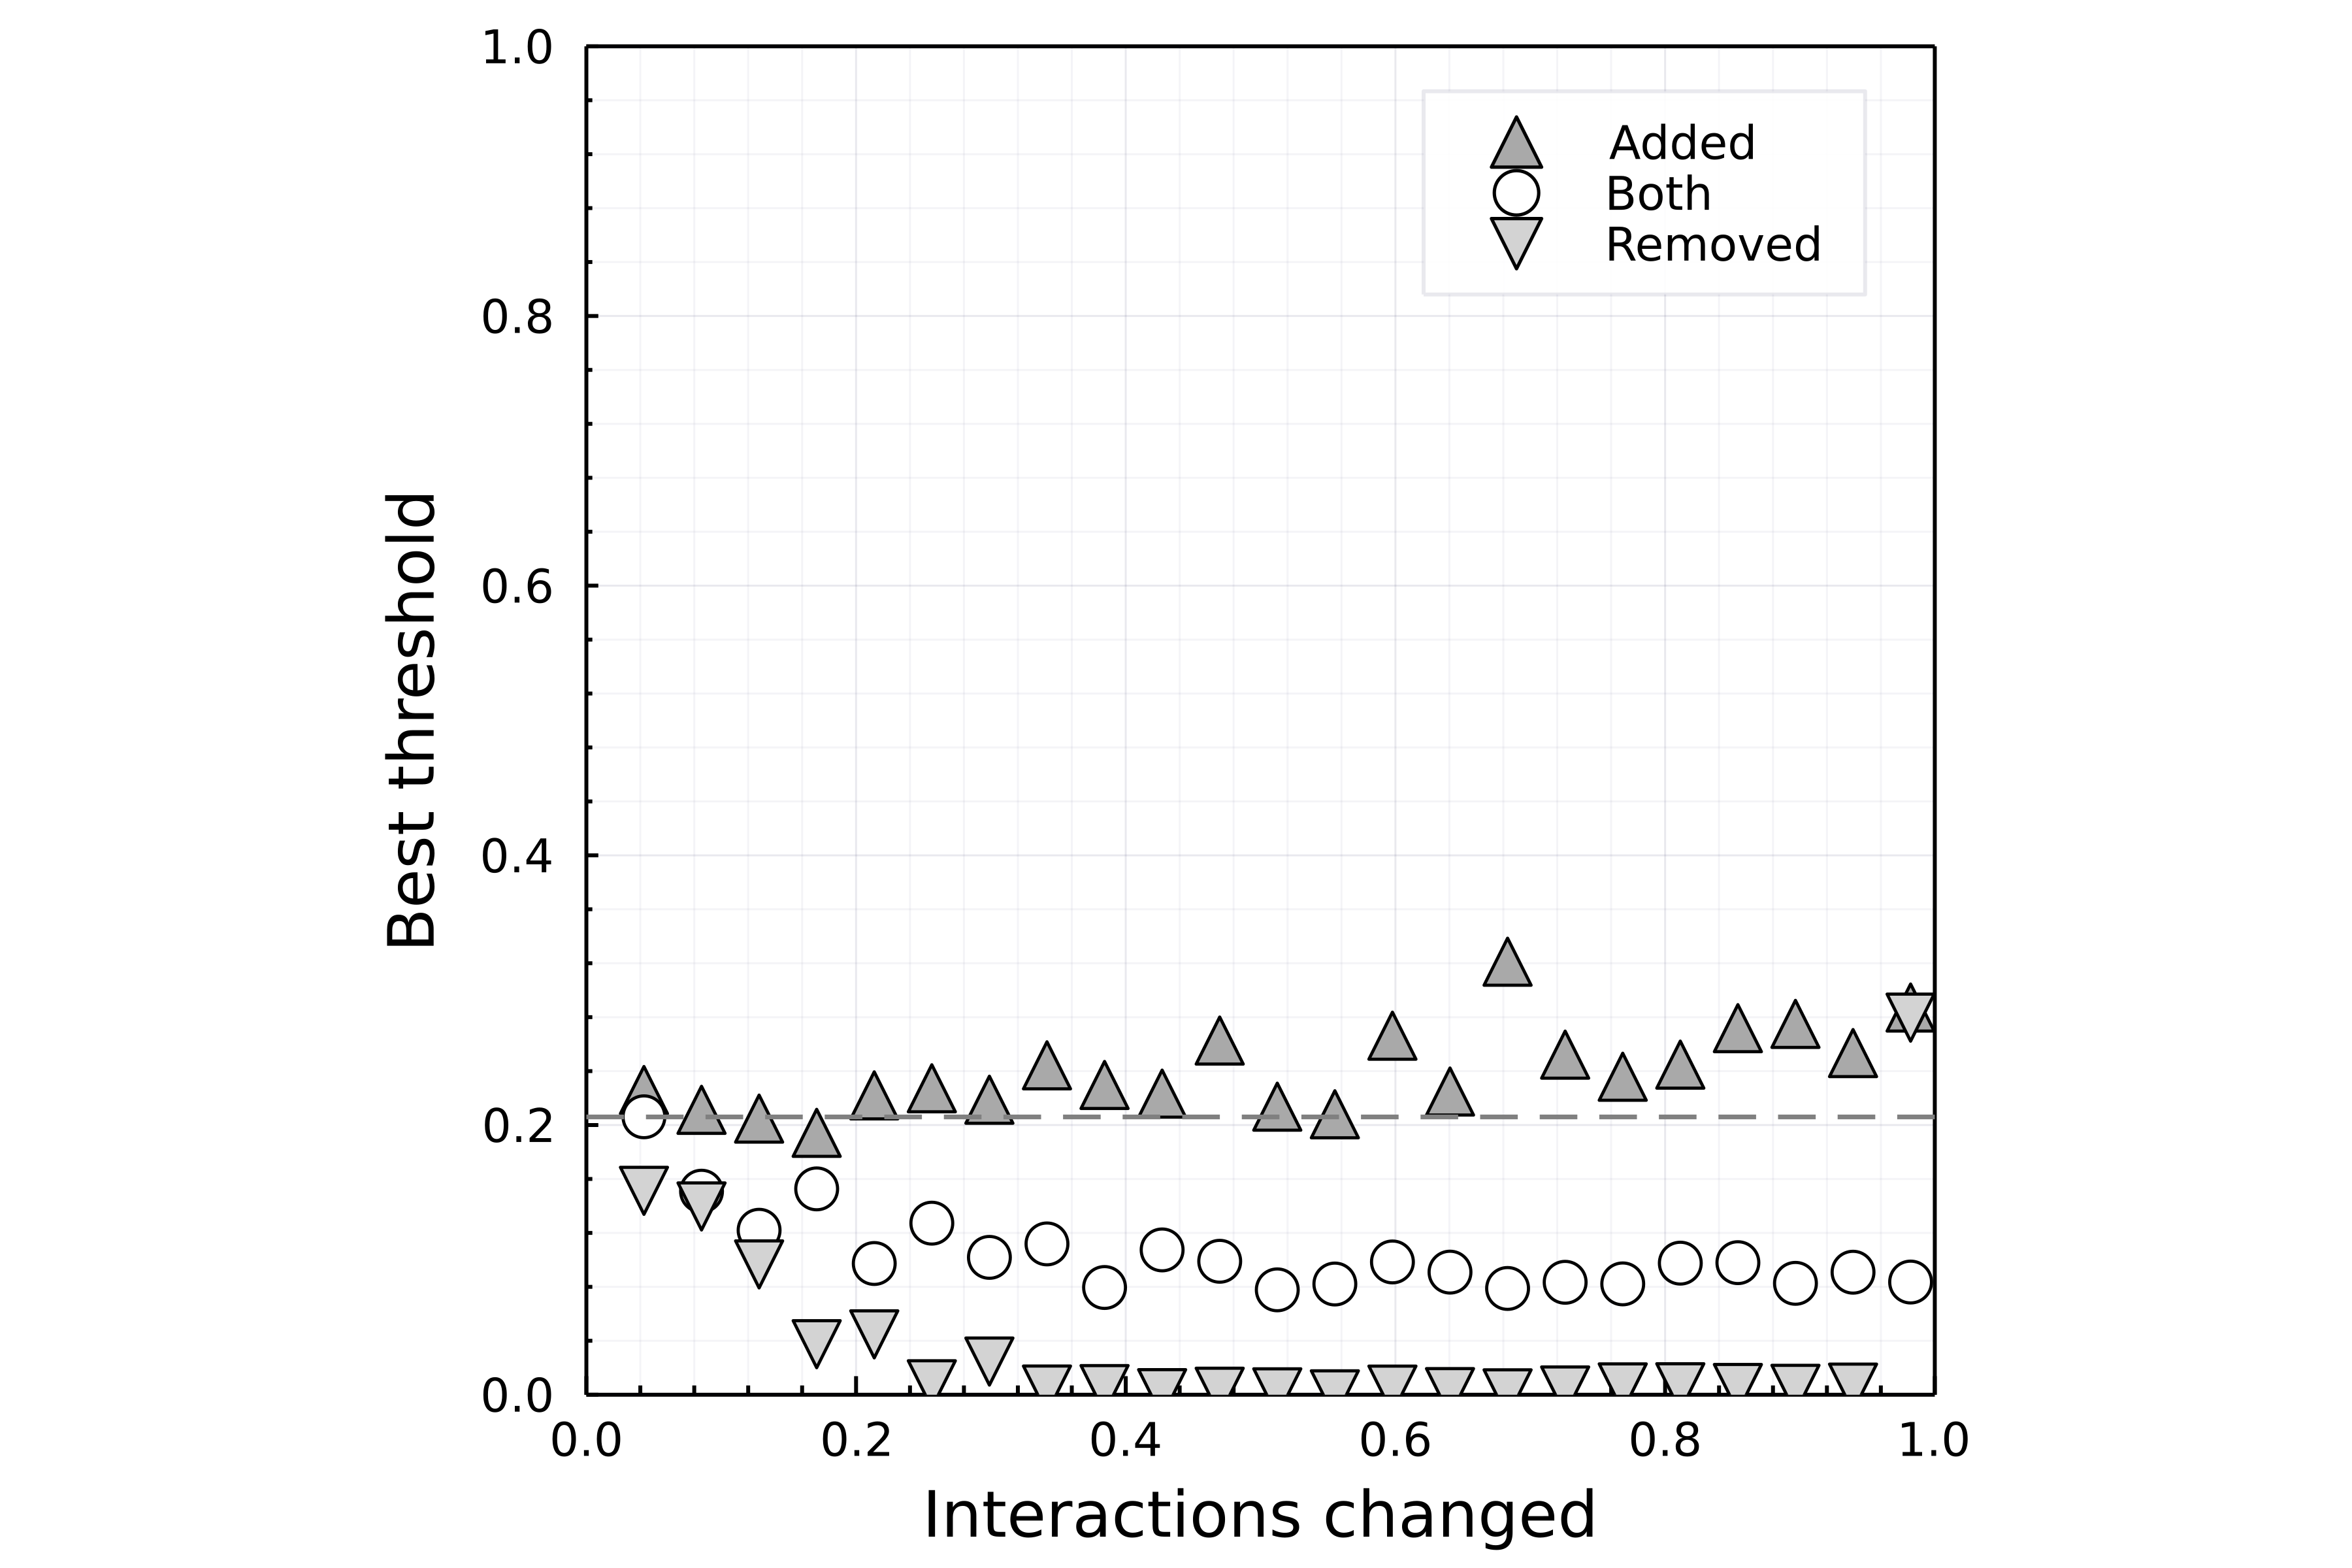
\includegraphics[width=\textwidth]{./figures/supplementary/sensibility_threshold.png}

The important consequence of this result is that training the RDPG on a
sub-sample of the network (\emph{i.e.} one missing interactions) would
result in a lower threshold, thereby potentially creating more false
positives when applied to novel data; this further justifies our
decision to use the entire evidence to estimate the threshold.

\subsection{RDPG yields an accurate
classifier}\label{rdpg-yields-an-accurate-classifier}

More important than the recovery of removed interaction is the fact that
the classifier should have a good global performance. One measure to
assess this is the area under the receiving operator characteristic
curve, or ROC-AUC. By this measure, the RDPG remains an excellent
classifier even if 50\% of interactions are withheld, and no matter what
the amount of changes are made by adding or both adding and removing
interactions.


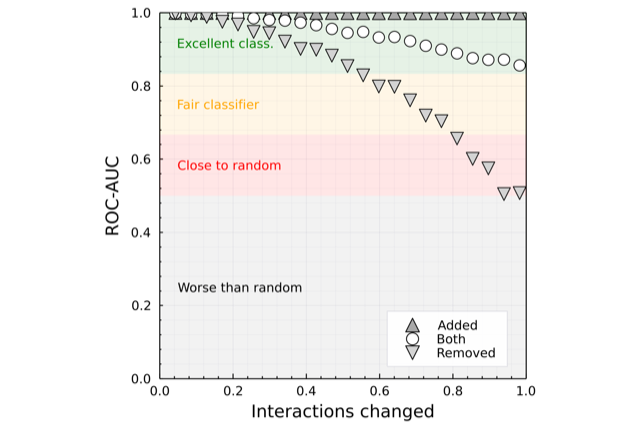
\includegraphics[width=\textwidth]{./figures/supplementary/sensibility_rocauc.png}

The overall agreement between a classifier and the actual data can be
measured by Cohen's \(\kappa\), which gives a similar result.

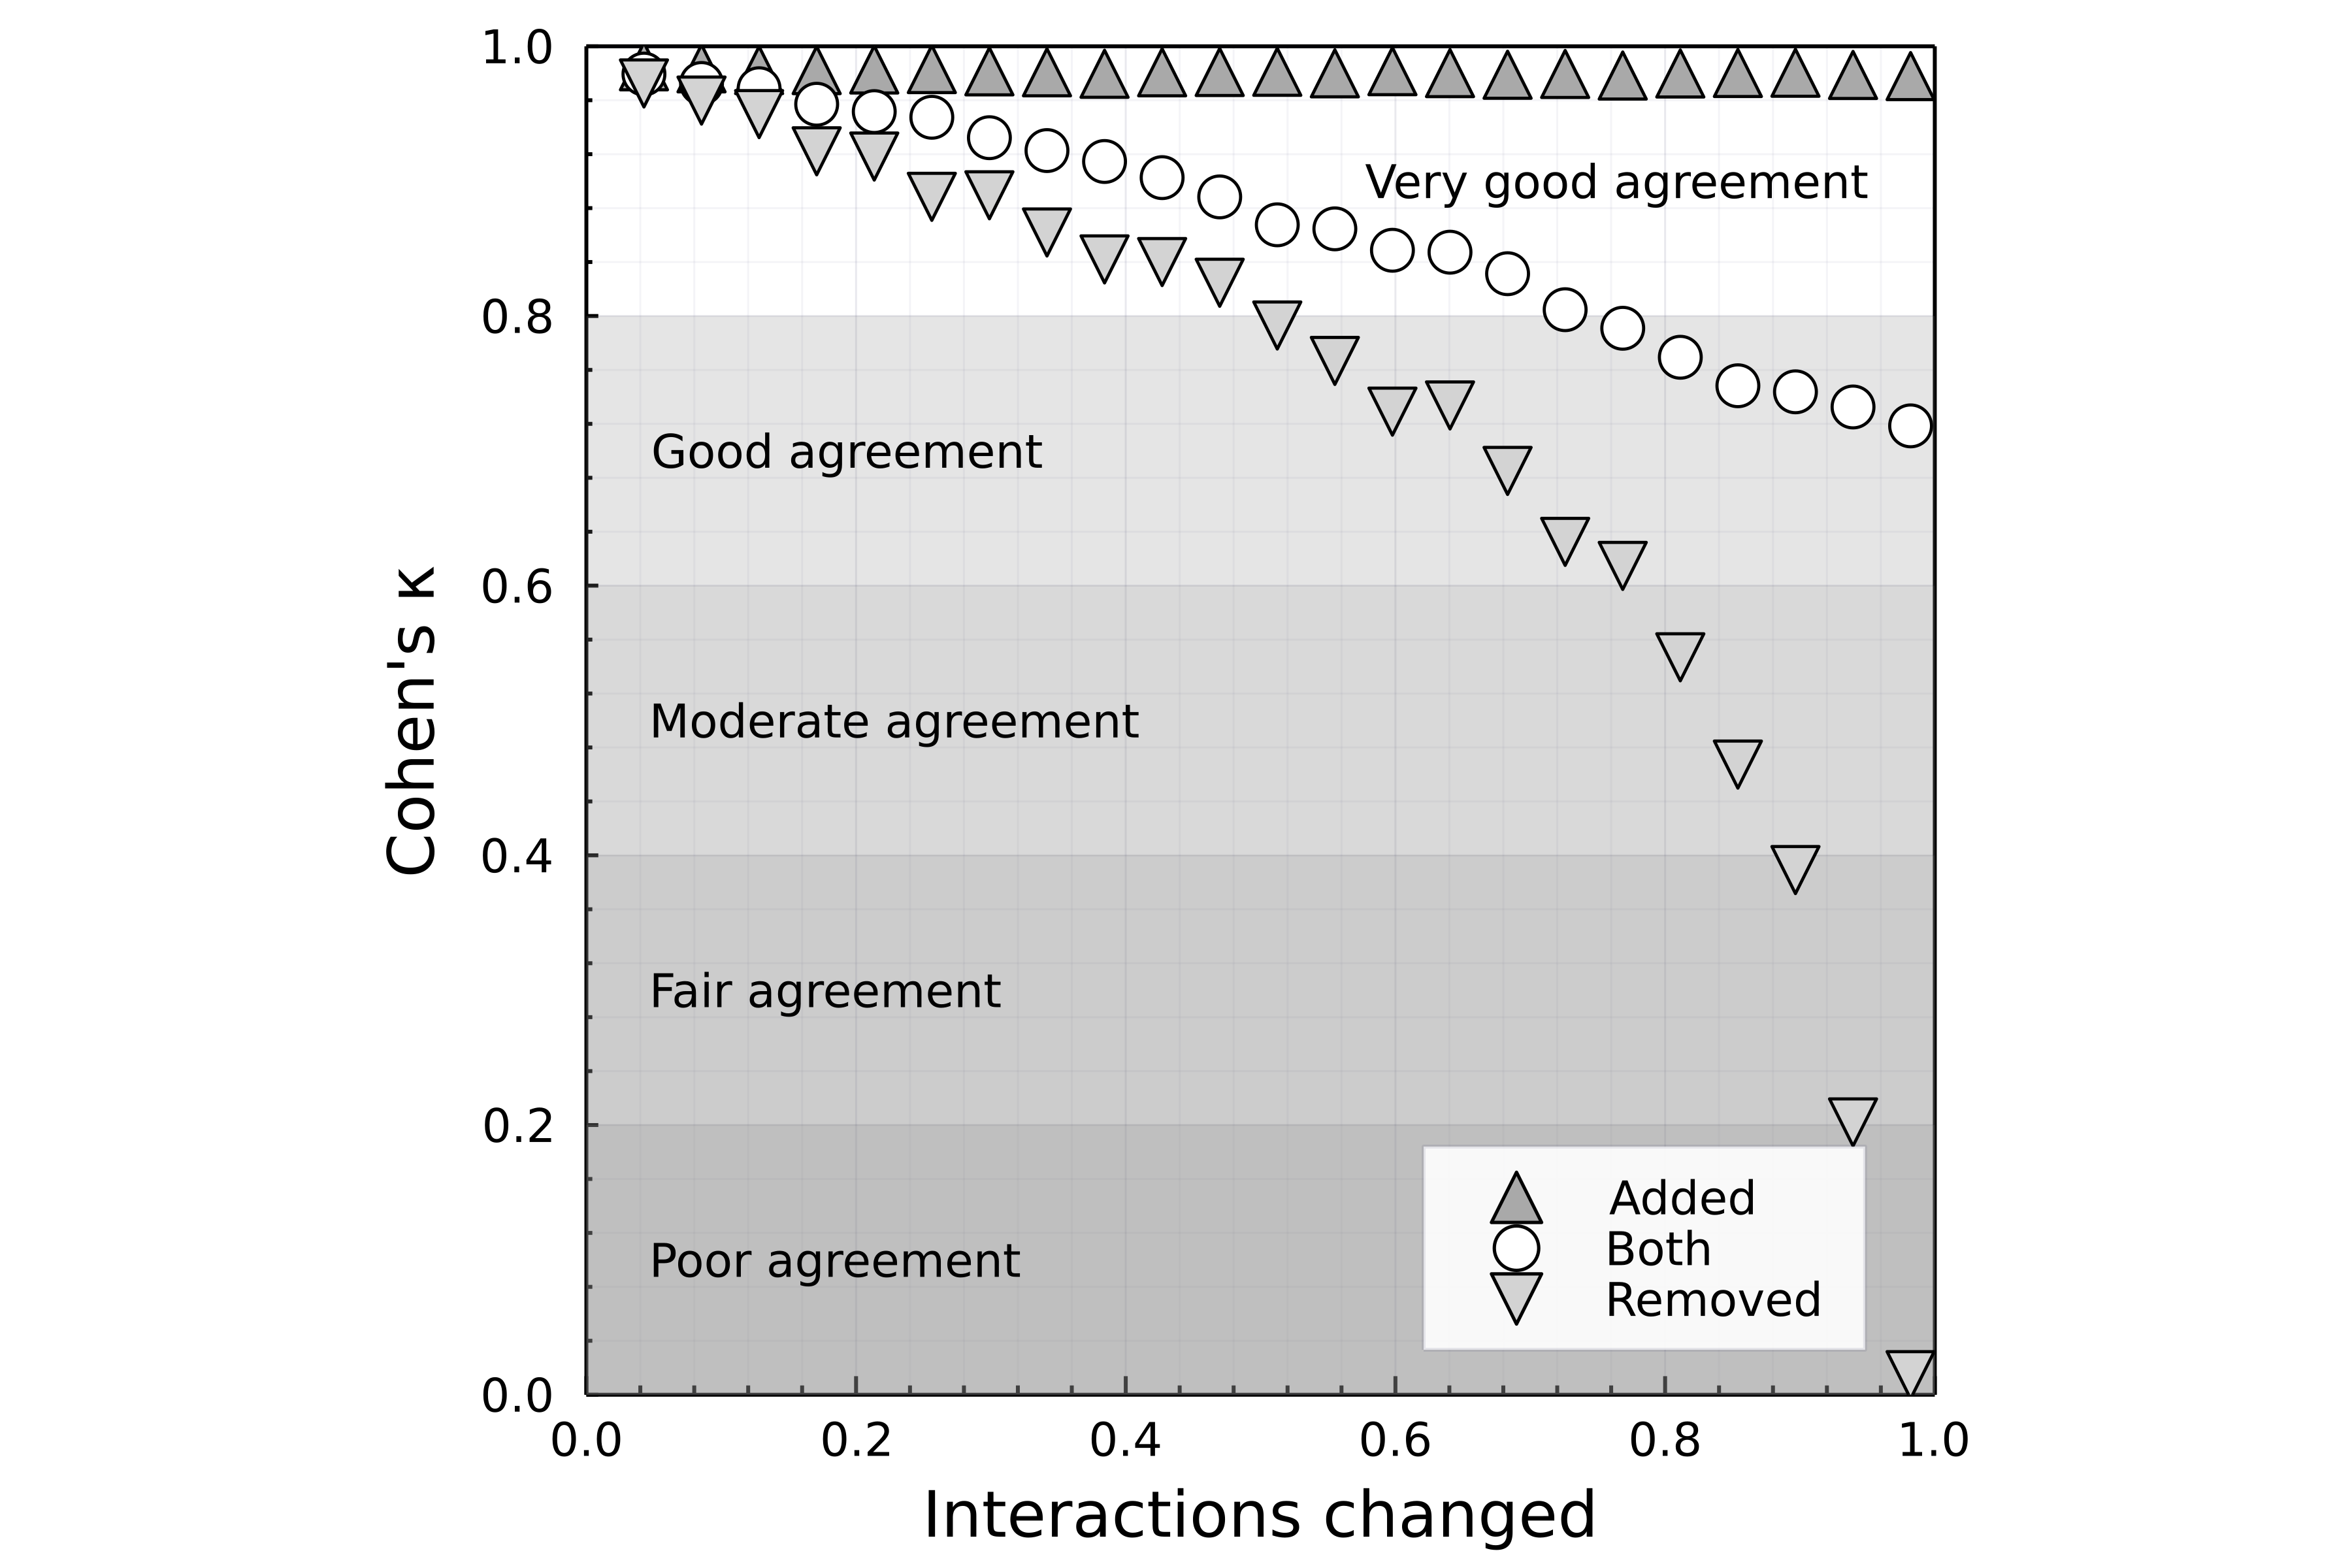
\includegraphics[width=\textwidth]{./figures/supplementary/sensibility_kappa.png}

These two diagnostic figures reveal that, although we used a probably
exhaustive list of interactions to do the initial RDPG, there are
chances that the approach would work on less complete datasets.

\subsection{RDPG recreates ecologically realistic
networks}\label{rdpg-recreates-ecologically-realistic-networks}

In this section, we present the relationship between the empirical
measure of the network structure (dashed line) and the reconstructed
estimate based on RDPG after the optimal threshold has been applied. We
focus on connectance (for its broad relevant to food web structure)
first:

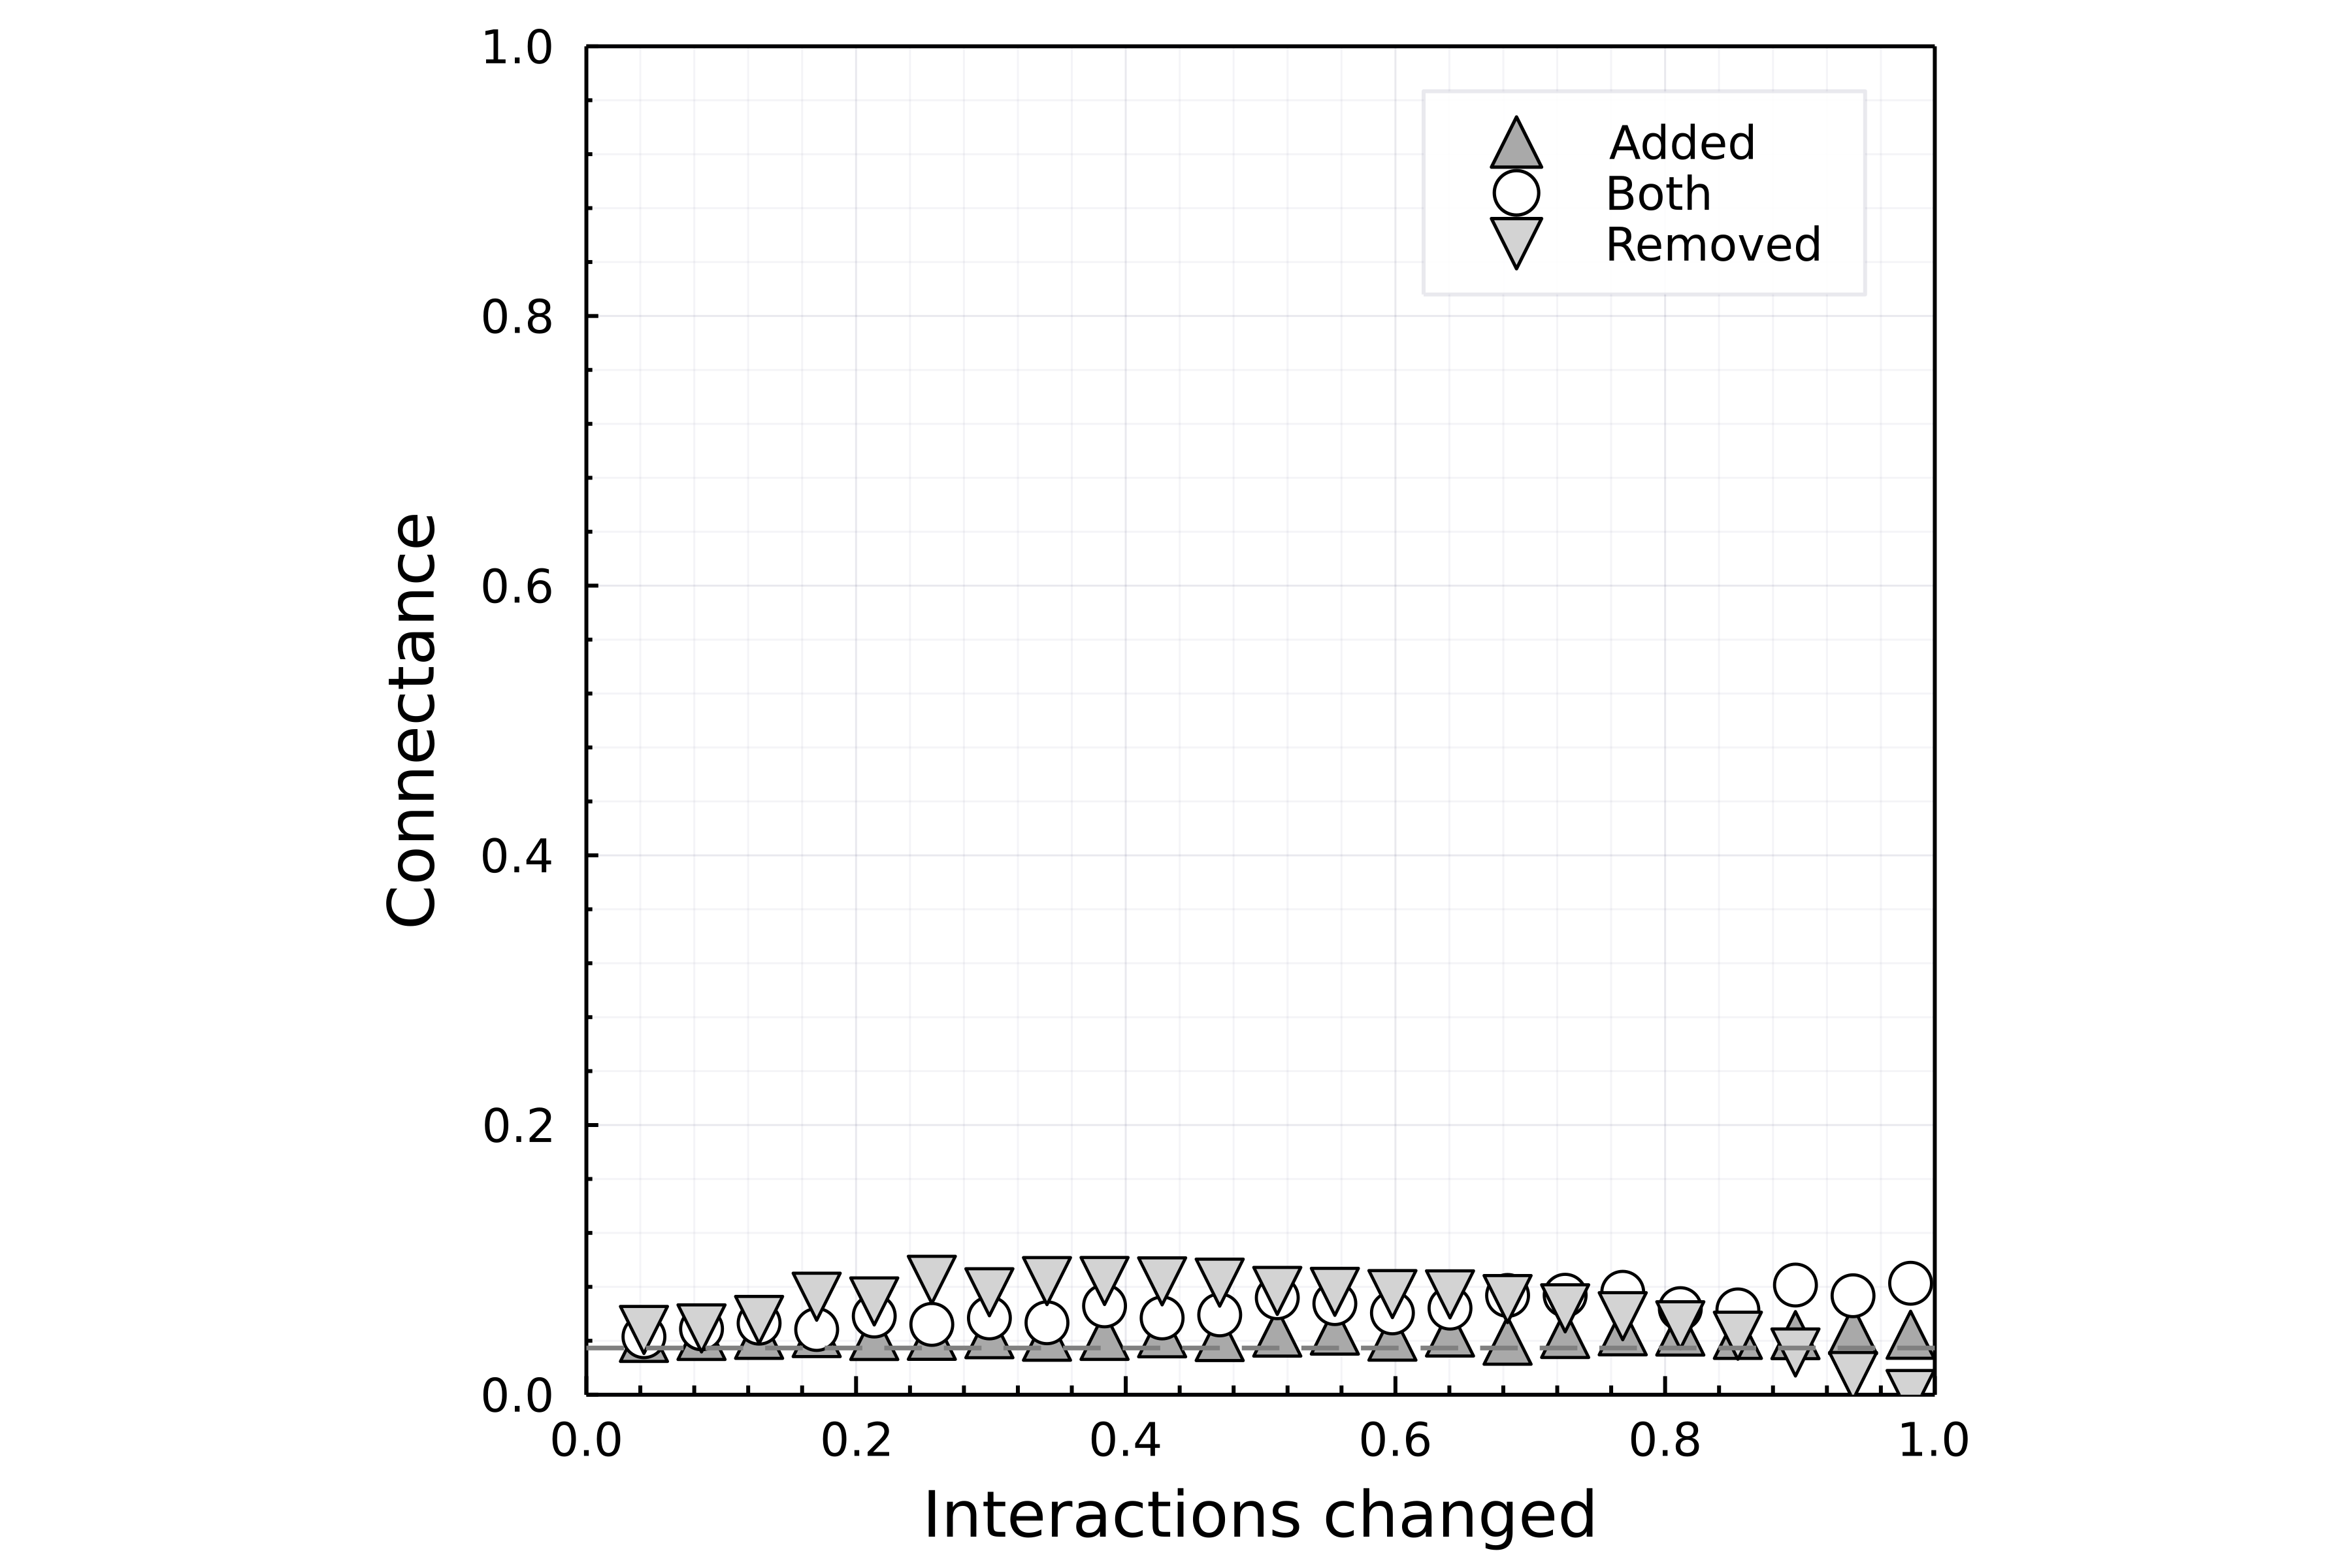
\includegraphics[width=\textwidth]{./figures/supplementary/sensibility_connectance.png}

Connectance increases slightly when initial information is incomplete,
but saturates at a value of around 0.12 -- this is still within the
bounds of connectances expected for food webs.

Next, we look at the ratio between direct competition
(\(a \rightarrow (b,c)\)) and apparent competition
(\((a,b) \rightarrow c\)) motifs, as motifs are known to be conserved
blocks in food webs:

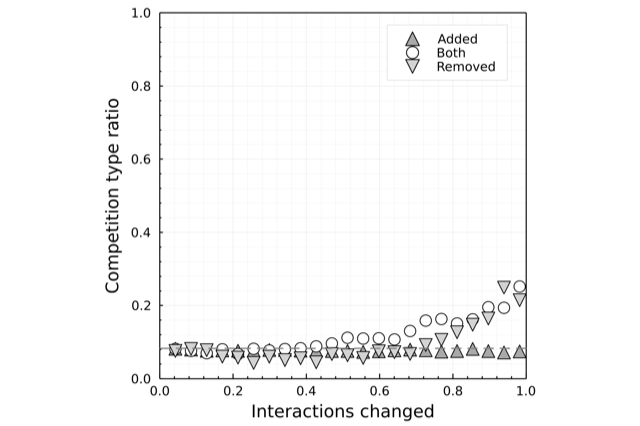
\includegraphics[width=\textwidth]{./figures/supplementary/sensibility_motifs.png}

This ratio remains close to the real one up until 75\% of initial
interactions are modified.

\subsection{Consequences}\label{consequences}

Based on these results, applying RDPG on the entire European network is
reasonable, especially since (i) the threshold is insensitive to the
number of withheld species, and (ii) removing interactions would
artificially lower the threshold. Interestingly, the RDPG remains an
excellent binary classifier even in the face of strong data
modifications, which suggests that our framework can be used even in the
absence of a complete metaweb. Even more importantly, the addition of
wrong interactions to the original dataset was never an issue for the
RDPG classifier, which was almost always able to remove them.

\section{The Normal model of latent variable evolution
over-predicts}\label{the-normal-model-of-latent-variable-evolution-over-predicts}

In this appendix, we compare the raw predictions made by the Normal and
Uniform models of latent variable evolution. The Normal model was
created by (i) getting the average \(\mu\) of the simulated values for
each species/variable combination, and (ii) estimating the standard
deviation as \((\mu+c - \mu-c)/3.92\), where \(c\) is one half of the
95\% confidence interval around \(\mu\) divided by 3.92

As can be seen on the following figure, the Normal model tends to assign
high probabilities (up to \(p \approx 0.4\)) for interactions that the
Uniform model essentially rules out:

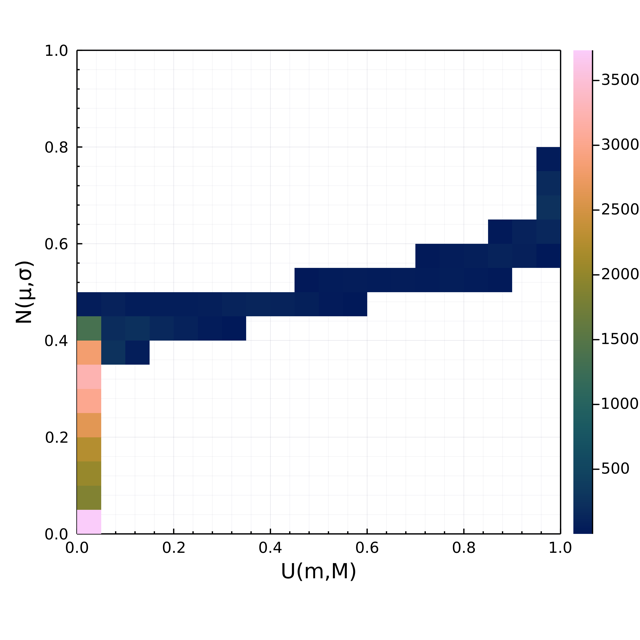
\includegraphics[width=\textwidth]{./figures/supplementary/comparison_models.png}

This can lead to severe over-estimation of the number of interactions.
In fact, the consequences of using a Normal model are obvious from
looking at the adjacency matrices below: most of the interactions are
predicted between species that occupy the lower trophic level, and are
ecologically unrealistic.

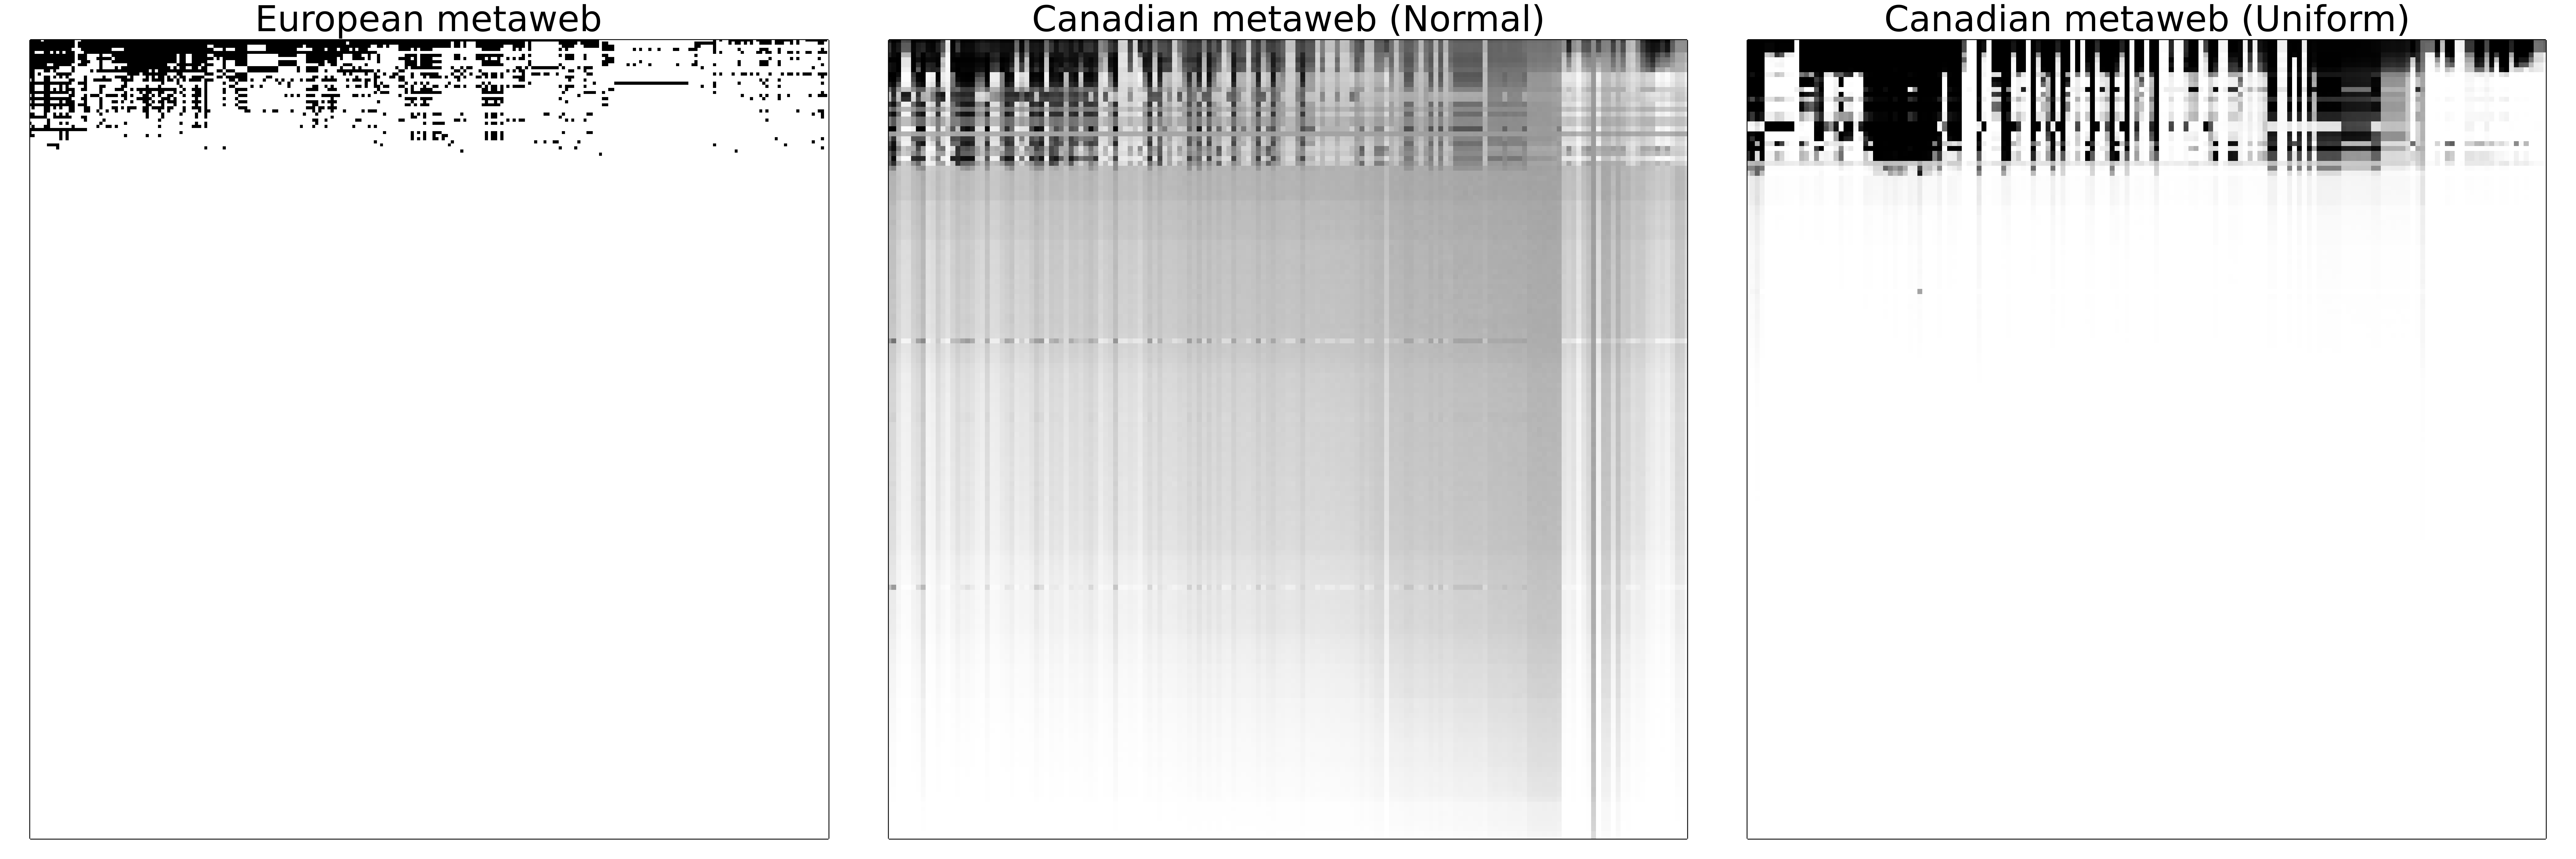
\includegraphics[width=\textwidth]{./figures/adjacencymatrices.png}

This can be further revealed by looking at the connectance of the
networks under different thresholds:

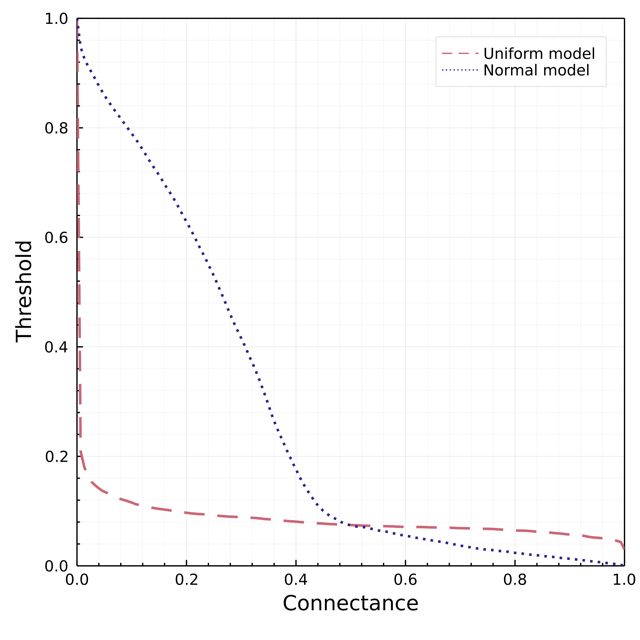
\includegraphics[width=\textwidth]{./figures/supplementary/comparison_connectance.png}

Although the Uniform model predicts a lot of interactions with extremely
low probability, that are removed at a low threshold, the distribution
of probabilities under the Normal model leads to extremely (abnormally)
high connectances even for thresholds that are over twice as large as
the optimal threshold determined in main text and Supp. Mat. 1.

This has consequences for the overall network \emph{structure}:
specifically, the Normal model predicts a lot more top predators than we
expect under the uniform model; rather than there being a progressive
change in top-intermediate-bottom proportions as the threshold changes,
there is an abrupt shift at a threshold of about 0.6, which suggests
that the Normal model is biased towards over-predicting most
interactions with probabilities in the range \([0,0.6]\).

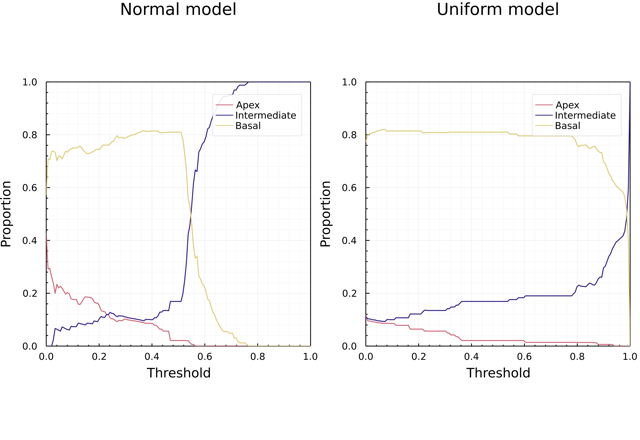
\includegraphics[width=\textwidth]{./figures/supplementary/comparison_tib.png}

The same ``jump'' can be observed when looking at the distribution of
food chain lengths:

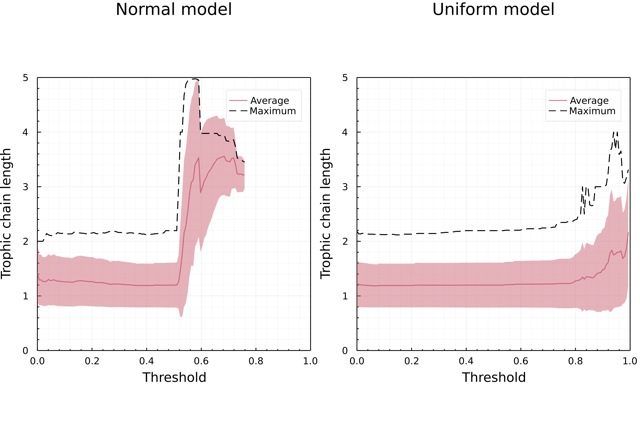
\includegraphics[width=\textwidth]{./figures/supplementary/comparison_rophicchain.png}

For these reasons, we only use predictions from the Uniform model in the
main text.

\section{RDPG reconstructed networks have diverse
structures}\label{rdpg-reconstructed-networks-have-diverse-structures}

In this appendix, we check that the networks reconstructed from the RDPG
do keep a variety of structural components, especially when selecting a
small species pools from within them. In order to do so, we induced 400
random subgraphs containing between 30 and 70 species, both from the
Canadian and European metawebs. For each of these subgraphs, we measured
eight variables: the mean and standard deviation of trophic levels, the
standard deviation of degree (total, in, and out), and the proportion of
top, intermediate, and basal species. We selected a random subset of 300
rows from the network-property matrix to fit a Principal Component
Analysis projection matrix (\(W\)), which we then used to project all
networks into the space formed by the first two principal components.

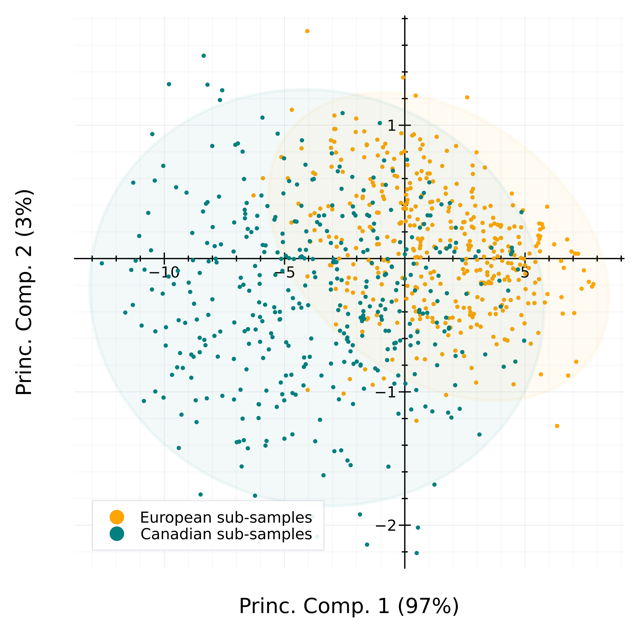
\includegraphics[width=\textwidth]{./figures/supplementary/variation_pca.png}

The first axis (explaining most variance) was strongly correlated to the
standard deviation of the number of preys (-0.71), and the second axis
to the standard deviation in the number of predators (-0.95). These
results match the conclusions in main text, namely that the first
dimensions of network embedding capture the degree distribution.

Two things are important to note on this representation; each point is
an induced sub-graph, and the ellipses are the 95\% confidence interval
around the points. First, there is some variations \emph{within} a group
(Europe \emph{v.} Canada); second, the two groups do not fully overlap.
This suggests that not only the sub-samples of the Canadian metaweb are
not equivalent to the sub-samples of the European metaweb (\emph{i.e.}
the two networks have structural differences), realizations (here in the
form of random local species pools) of the Canadian metaweb also show
some variability; in short, reconstructing a metaweb using a RDPG will
not result in homogeneous local networks, and may therefore be suitable
for lower-scale predictions.